\chapter{Methodology}
In this thesis we wanted to get an in-depth understanding  of the relationship between elderly, video games and exercising, in addition to observe how elderly interact with existing video games aimed for exercising. We wanted to learn this to build up under the concept we were developing. Often a project falls under one of two research methods, either quantitative or qualitative.  In this thesis  different qualitative research methods are used because this method allows us to get an in-depth understanding of a phenomenon. Observation and focus group interviews have been widely used, in addition to support methods like video recording and audio recording. Observation studies are often characterize by "naturalism", meaning that the "world" to be studied should be studied in its natural setting \cite{tjora}. In this project, however, we are studying a fixed setting, which was realised by experimental simulation.  We have called the complete session, including the observation of the experimental simulation and the focus group interviews a workshop, because we found this to fit well under the definition which is "A meeting at which a group of people engage in intensive discussion and activity on a particular subject or project" \cite{dictionary}. In this chapter we will describe the different research methods we have used, and how they have been conducted in this project. In addition we will discuss some of the limitations and challenges with the different methods. We will begin by describing which research strategy we have used to choose a setting for our study. 

\section{Choosing the Setting for Our Study}
 When doing research there are three criteria you would like to maximize \cite{McGrath}: 
 
A: Generalizability, \\
B: Precision, and \\
C: Realism.  

However, it is not possible  to maximize all three criteria because if you do something to increase one criteria, you are likely to decrease an other criteria. In our study realism is the most important criteria and is the one we want to maximize as much as possible.

There are different research strategies that can be used. Sometimes it is hard to find one that fits exactly to what you as a researcher want to do.
\begin{figure}
\begin{center}
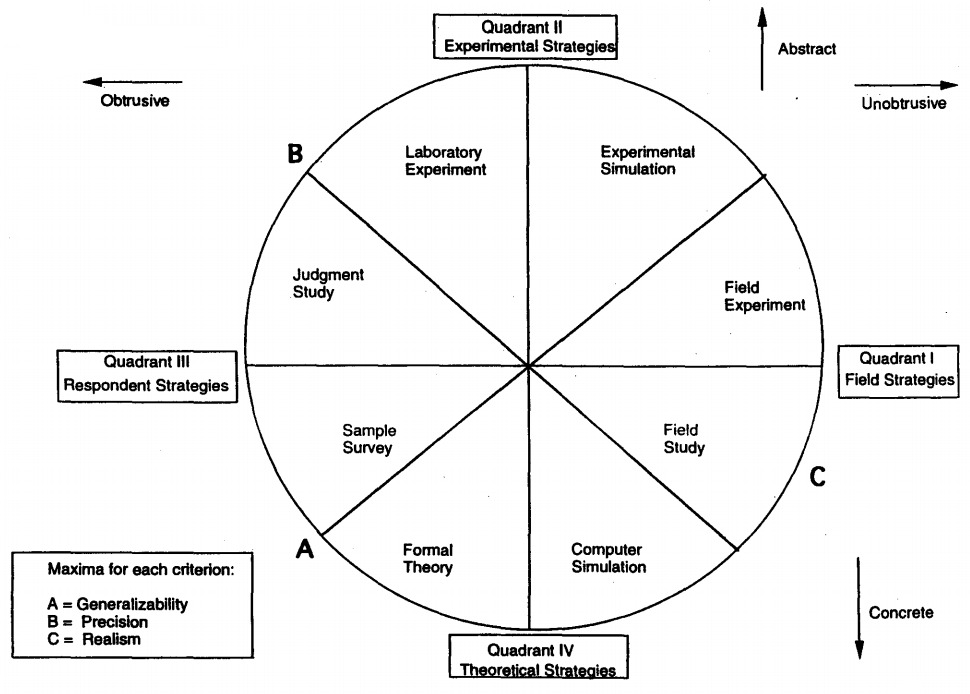
\includegraphics[scale=0.5]{circumplex}
\caption[The strategy circumplex]{The strategy circumplex \cite{McGrath}}
\label{fig:circumplex}
\end{center}
\end{figure} 
The strategy circumplex, shown in Figure \ref{fig:circumplex} shows eight different strategies \cite{McGrath}. As can be seen from the figure the different strategies are arranged in a way on whether they are abstract versus concrete, and obtrusive versus unobtrusive. The figure also shows at what strategy the three different criteria, A, B and C, are at their maximum. We studied this circumplex to find where our study fits in. We found one of the strategies from quadrant 2 appropriate. Within this quadrant there are two different strategies, laboratory experiment and experimental simulation. In the former strategy the researcher put together a setting and invite some individuals to enter the setting and act by the defined rules. Here the researchers typically know what behaviour they are looking for and can within this setting study this with precision. The second strategy is experimental simulation. At the same time as trying to get the precision, as in a laboratory experiment, the researcher also try to get some more realism as in the strategies in quadrant 1 do. This means that the researchers are setting up a situation like in the laboratory experiment, but at the same time are trying to get some realistic behaviours from the participants. This means that the researchers try to get sufficient realism, and at the same time keeping sufficient precision and control. The field experiment strategy within quadrant 1 was also considered because we found it in some ways to fit for our study. This strategy, compared to field study which has maximum degree of realism, opens up for being a little more obtrusive, and in that way give up some of the realism. We wanted to create an as natural setting as possible, and to implement the study in a place familiar to the informants. However, as defined in \cite{McGrath}:  "The essence of both of the strategies in quadrant 1, the field study and the field experiment, is that the behaviour system under study is "natural", in the sense that it would occur whether or not the researcher were there and whether or not it were being observed as part of a study", which means that our study does not fit in within this quadrant. In contrast, the behaviour gotten from the two strategies within Quadrant 2, would not have been apparent if it was not for the researchers doing the study. Therefore, we conclude that we in our study uses some variant of experimental simulation, even though no study is fully under only one strategy. It is important to understand that even though experimental simulation is less realistic, the study is still real and the behaviours gotten from the participants are real, however influenced by the setting \cite{McGrath}. Because the experimental simulation never can be as realistic as the field study, there will be an error in the information gathering, which can pose validity issues \cite{alsos}. This will be discussed in more detail in Chapter.. First we will discuss the research methods used to gather data from the experimental simulation. 

(As a primary research strategy we used experimental simulation in our study.  As information gathering methods we used qualitative research with observation, video recording and focus group interviews.  As an additional support method, we used surveys. This was done to in an efficient way gather information about  who the informants are, and their attitudes towards exercising in general, and technology in general. We will not discuss the different research methods used. )


\section{Qualitative Research}
Qualitative research is a method used to get an in-depth understanding of a phenomenon. This research method is well suited when studying sensitive and personal topics, as well as when studying topics that there have not been done much research on. Interpretation is very important in qualitative methods, as well as flexibility and openness. The focus lies on how and why things are done, and not how many who does it, like in quantitative methods. Quantitative methods include huge samples, while qualitative research can give more information about a small sample \cite{qualitative}. This often result in a close and personal relationship with the people being studied \cite{tjora}. In quantitative methods structuring is very important, while flexibility is important in qualitative methods. With flexibility it means that the scheme should have the possibility to be changed during the research, if needed. Another aspect different from quantitative research is that it is not common to use numbers, because the numbers would be too small \cite{qualitative}. \\ \\
The qualitative research process can be divided into phases, that partially overlap. The first phase consists of defining what the research will find out. We have done this be defining some research questions. The next phase is the data gathering phase. This phase can be performed with different methods, discussed later. The next phase includes interpreting and analysing of the data, as well as formulating theories. In the last phase, the results will be presented. Data gathering and analysis should be done in parallel. In that way, further data gathering can be adjusted from what have been found in earlier analysis. There are four different data gathering methods described by Thagaard in \cite{qualitative}:

- Observation \\
- Interview \\ 
- Document analysis, and \\
- Analysing of video and audio recordings

The most common methods are interviews and participatory observation. These are primarily the two methods we have used in our thesis. It is common in qualitative research to have a close connection between the researcher and the people who is being studied. This especially apply in interviews and observation. This contact is important for the data the researcher will gain from the study \cite{qualitative}. The interview method and the observation method will be described in more detail later in this section.

In most qualitative methods it is common to textually document the data which is being analysed. The documentation can include what people do, their statements, their intentions or their perspectives. The text can be notes from the field or printouts of  recorded interviews \cite{qualitative}. In this thesis, these documents will be provided in appendix.

\subsection{Ethical Challenges}
The close contact established between the researcher and the informants introduces some ethical challenges. All results conducted from the research needs to be precisely and correct when presented. This also includes other researcher's work. Plagiarizing means to copy other people’s work and take credit for it. This is illegal, and it is therefore important to properly state the resource of the information that is being presented.  When working in close contact with informants, the researcher often gets personal information about the informants. With personal information we mean information that can be linked to individuals. In projects with this kind of information, the project needs to be reported. In the case of research projects performed at universities, the project needs to be reported to \ac{nsd}, which is an entity in care of data protection for these institutions. \ac{nsd} will evaluate each project in accordance to research ethical rules \cite{qualitative}. In this thesis we will do observation of a fixed workshop, as well as focus group interviews with the participants of the workshop. This will require having a close connection with the participants, as well as gather personal information about them. In addition, we will video record the workshop and audio record the interviews. Therefore, this thesis has been reported to \ac{nsd}, see Appendix X. 

\subsubsection{Ethical Guidelines:}
Tjora \cite{tjora} suggests that common politeness should be a basis for ethical research. However, some additional rules needs to be followed. These are described in the following guidelines:

\emph{Informed Consent:} \\
In a research project with people involved, there is a requirement that the researcher has the participant's informed consent. This means that the informants have gotten all the information they need to know about the participation, have self chosen to participate, and that they can withdraw at any time without any consequences. One challenge about this, is that in some projects too much information can affect the participants behaviour (for example if the participants know too much about what the researchers are looking for, they can act differently) \cite{qualitative}. In this thesis we do not see this as a problem, and the participants were well informed of what we were researching. To get participants to our study, we contacted the manager of "Seniornett", which is a group of seniors that is interested in learning about technology. Once a month this group has meetings with different topics each time. We was invited to present the topic of exercising with video games in one of this meetings. After this meeting, we invited the ones being interested, to participate in a workshop. In this way, all the participants got a thorough description of the project we were working on, as well as how the workshop would be conducted. In addition, every invited participant, got an invitation letter, with a short description of the project and information about what they were going to participate in, and their rights. Every participant gave us their written consent to participate. The presentation, invitation and written consent can be found in Appendix Y.   \\ \\
\emph{Confidentiality:}\\
Researchers are required to keep all the information they collect about a participant confident. This means that the information have to be anonymized. This also involves strict requirements to how personal data, that makes it possible to identify individuals, should be stored and annulled. There are rules about how long data can be stored. General principles are that data should be stored for only the amount of time it is use for the data, and that data which can be directly linked to an individual should be stored separately and not electronically.  Reuse of data is not allowed without consent from the participants \cite{qualitative}. In this thesis we have signed a non-disclosure agreement to assure the participant that we will not reveal any confident information about them. This is found in appendix Z. In addition, we have assured the participant that all data we collect will be deleted within 3 years after the project's end. See Appendix Y. \\ \\
\emph{Consequences of participating in research projects:}\\
The researcher has responsibility over the participants safety and should respect their wishes. It is important to have thought through what consequences the execution of the research have for the participant. The researcher is required to protect the participant's integrity during the process \cite{qualitative}. In our workshop, every participant was allowed to choose what they were comfortable with doing and not doing. They were allowed to withdraw at any time without any consequences.  \\ \\
\subsection{First Phase} 
The first phase in the qualitative research process is to define what needs to be found from the research. A problem description (research questions?) should be prepared and a design for how the research will be performed should be developed. The design consists of guidelines of how the project should be carried out and includes: \emph{what} the study will focus on, \emph{who} are the informants, \emph{where} the study will be performed, and \emph{how} the study will be performed. Our design will be described in detail in the next chapter. Vet ikke om vi skal ha med noe om prosjektbeskrivelse (ikke det samme som problem description.. det er problemstilling)? det går på hvem som skal jobbe, hvordan finansiere osv..A problem description needs to be developed in order to know what the study should be focusing on. This will contain research questions the researcher wants to get information about. The problem description should be clearly prepared and it should be limited realistically within the framework of the project, and at the same time be open enough so that new, interesting topics that appear during the process can be studied. It is also important that the problem description is being modified and worked with during the research process, because the researcher will gain new knowledge and understanding during the process which can be important for the research. The choice of problem description should be justified by describing why the problem the researchers will study is important \cite{qualitative}. The research questions are described in the next chapter. 

\subsection{Observation}
Observation, often called ethnography \cite{tjora}, is used when the researcher wants to see how a group of people behave in a specific setting \cite{qualitative}. With observations the social world will be studied in its natural setting, to get a real and natural view of the world. There are several good reasons for choosing observation as a research method. The researcher can observe social settings, that the actors in the setting never before have interpreted themselves, and the researcher can understand what people actually do, instead of just getting what the people say they do (like in an interview) \cite{tjora}. When doing observation, one important decision is how the observer will perform in the field. This varies from project to project. The observer can be a participant or just an observer, and the observation can be open or undisclosed. Participatory observation is something in between being a complete observer, where the researcher keeps himself in the background, and complete participator, where the researcher participate in the same way as the informants. This involves the researcher being present in the setting of the participants while observing how they act. The researcher participate in the session, in the sense of interacting with the participants while they are performing the tasks. This means that the researcher does not do the same as the participant. Participation observation is well suited in research of a new and immature topic \cite{qualitative}.

It is very common to combine observation with interviews. This is for the researcher to verify or discard the understanding he or she has acquired during the observation. In most research it is important to study the behaviour in the informants own environment. This will give a more natural behaviour. However, it is important to acknowledge that the informants may not find the environment "natural" when the researchers are observing them. How the researcher presents the project to the informants is important to gain interest among the people they want to observe. The researcher should in a trusting way, present him or herself and the project \cite{qualitative}.

In this thesis we have used observation as a method for understanding how seniors interact with commercial Xbox Kinect games. This does not fall under the immediate understanding of the definition of observation, as this is to gain understanding of "a natural world" \cite{tjora}. This is rather a future scenario. The planned exercise game was in our previous study \cite{project} evaluated to suit well into a clinical setting at the physiotherapists office, or/and in a group training session. Therefore, we tried to create an as realistic small group training session where 4 people played alone and together.  We wanted to see how the seniors where interacting with the game, as well as their reactions to different events. The workshop was held in the premises where the organization "Seniornett", which they all were members of, have their meetings. We did this, to make the setting as natural as possible.  However, in this case, it was not a natural environment where they "normally play a game", as none of the participants had played these kind of games before. This is why we have defined this session as an experimental simulation. We evaluate the setting, to be as natural as was possible at this time.  During the observation we looked for things that supports what we have read in the literature, as well as for new aspects that we were not aware of (see our research questions described in chapter..). This was for us to get an understanding of what works, and what does not work with existing commercial Kinect games. This was used as a foundation for the development of a new game concept. 

\subsubsection{Video Recording}
The workshop was video recorded. An advantage about using video as a tool for observing a situation is that you get a detailed representation of what happened in the situation. Together with the field notes taken, this will give a close to complete representation of the situation \cite{tjora}. To get a as realistic rendering of the situation as possible, it is important to decide the right camera angle. The quality of the recordings will also have an important impact on the data you get from it. Therefore, the video recordings have to be seen as one of more possible representations of a situation.  The fact that video recording gives the researcher a detailed representation of what happened is an advantage because it gives the researcher the opportunity to look through the recordings and see the situation again. In this way, events that the researcher might have missed during the observation, can be discovered. Video recording is also a useful tool in a situation where the researcher is unfamiliar, and when they do not know what they are looking for. The sociologist Hubert Knoblauch came up with the term "videography", which comes from the fact that video observation can be looked at as a form for ethnography with the use of video \cite{tjora}. Videography usually has a shorter data generation period with high data intensity, while traditional ethnography has prolonged periods.  While traditional ethnography often seek to get a wide understanding of social groups or settings, videography has a more sharpened interest in for example interaction, social situations or specific events. With the use of video, the researcher can focus more on the details. Video observation makes it easier to do the data analysis together with other researchers. The fact that more people can work together in a workshop can make the quality of the research stronger, giving more diversity, as well as detailed, complete and accurate interpretation \cite{tjora}.

It is always a risk that the people being observed will behave differently because they know they are being observed. This is called the Hawthorne effect \cite{interview}. This may have an even bigger impact with the use of video recording, and it is therefore important to remember this when analysing the data. The observers can also be affected by the situation \cite{tjora}. 

In addition to the observation, we arranged focus group interviews to verify or discard some of the things we observed, as well as discuss the participants' experiences with the video games. We will now describe in more detail the use of qualitative interviews.  

\subsection{Qualitative Interviews}
Interviews are typically used when a researcher wants to get comprehensive information about peoples views and opinions about a topic. Interview is one one of the most important tools used in qualitative research \cite{interview}. There are two extremities in interview methods: unstructured and structured interviews. The former is more like a conversation between the researcher and the informants. The topic is chosen, but there are no interview guide involved. In that way questions can be adjusted during the interview. The latter has a structured form, with chosen questions. The advantage with this method, is that all informants will answer the same questions, and therefore the answers can be compared. The third, and most common, type of interviews is semi-structured interview. This method is something in between the two extremities and is commonly called qualitative interviews \cite{qualitative}. This method includes a interview guide, where some questions are decided beforehand, but the order in which the questions are asked is chosen during the interview. In this way it is easier to follow the story of the interviewee. In addition, the researcher needs to be open to discuss other topics that might appear during the conversation. The most common interview setting is with one individual at the same time. However, group interviews, or focus groups, are becoming more common. In a focus group interview, several people discuss a topic, while the researcher(s) serve as a moderator. This can be more effective, because more data can be gathered at the same time. Sometimes it can also seem less intimidating for the informant, as they are discussing topics, instead of having a in-depth interview alone. In a focus groups the informants discuss with each other, which opens up for more data for the researcher. When discussing topics with other informants, they can give more spontaneous answers. The informants stimulate each other, which can give more aspects of the informants experience. In addition, this stimulation gives a source for new thoughts and reflections \cite{tjora}. 

\cite{tjora} discuss how a focus group can be organized.  A basic rule presented in the book is that a session should last for 1 to 2 hours, and have 6-12 participants. But there can also be mini-focus groups with 3-4 participants. Usually in the latter setting, the participants are experts on the topic. In a focus group, one or more moderators are used to lead the discussion, take notes to be able to follow up topics that appears during the session, and to come up with new topics \cite{tjora}. To get a successful interview, it is important that the researcher has an understanding of the informants’ situation for the questions to be relevant. Questions should be asked in such a way that the informant can reflect over the question and not only answer "yes" or "no" \cite{qualitative}.

In this thesis we have performed focus group interviews with 4 participants after the play-session. The interview was semi-structured or qualitative, where we had some predefined questions, but at the same time held the conversation open, so new topics that would arise, could be included. The questions were developed from from what we learned from the literature to be important aspects to find when developing video games in general, and for this user group. In addition, the questions were adjusted to what we observed during the workshop. 

\subsubsection{Audio Recording}
To report all the data we got from the interviews, we used audio recording. This was for us to be able to get everything that was being said, and at the same time concentrate on the conversation. When audio recording is used, it is necessary with a complete transcription of the material after the interview is finished. One smart rule is to always transcribe a little bit more detailed than what the researcher think is necessary. When going from audio to textual presentation, there is common to lose some visual ques, as well as the tone in the interview \cite{tjora}. However, if the same researcher performs the interviews, the transcribing and the analysing, he or she will most likely remember the different event. This was the case in our interviews, and is therefore not seen as a limitation. 

\subsection{Possible Pitfalls}
There are some possible pitfalls when doing qualitative research, especially when doing qualitative interviews. We will discuss some of them that can have affected our interviews here based on a list discussed by Myers and Newman in \cite{interview}: \\ \\
\emph{Lack of trust:} We did not know any of the participants. This can have affected our trustworthiness. This may have resulted that interviewees held back important information, which would make our data gathering incomplete. In addition, the participants did not necessarily know each other, which also may have affected how they answered. However, in this case, all the participants had voluntarily chosen to participate, as well as gotten a non-disclosure guarantee from us. The topics discussed will not classify as very personal. Therefore, we believe that this has not affected our data.\\
\emph{Lack of time:} We were restricted by a time limit.  Time limit can give both positive and negative results. It can lead to incomplete data gathering, because of lack of time to ask all the questions we wanted. It can also result in more data, because the interviewee under time-pressure  may quickly have created opinions. However, this data may be less reliable. Both the group interviews were finished before the time limits were out, and did therefore believe that this did not affect our data.\\
\emph{Constructing Knowledge:} Interviewees may be asked questions that they have never reflected over before. This may lead to the construction of stories for them to appear knowledgeable. As this was a interview more about the the experience about the gameplay, and not so much about knowledge, we believe that all the answers were real. \\
\emph{Ambiguity of language:} A word can have different meanings. This can be misunderstood by both actors in the interview. With the participants' lack of experience with this kind of technology some words were unfamiliar for the participants. We were very aware of this, and feel that we in a natural way managed to ask questions at an understandable level.\\
\emph{Elite bias:} The interview can give incomplete and under-representative data if only one type of group is interviewed. It can then be hard to understand the broader situation. Because of time limit and practical reasons, we only included one group of people with the same interests for learning and keeping up with technology. Our data gathering would probably be different, if we gathered a group of "random" people, because they would have different backgrounds and interests. This will be discussed in more detail in Chapter (discussion).



